%%%%%%%%%%%%%%%%%%%%%%%%%%%%%%%%%%%%%%%%%%%%%%%%%%%%%%%%%%%%%%%%%%%%%%%%%%%%%% %%%%%%%%%%%%%%%%%%%%%%%%%%%%%%%%%%%%%%%%%%%%%%%%%%%%%%%%%%%%%%%%%%%%%
%
%
%
%	1. Motivation
%
%
%%%%%%%%%%%%%%%%%%%%%%%%%%%%%%%%%%%%%%%%%%%%%%%%%%%%%%%%%%%%%%%%%%%%%%%%%%%%%%%%%%%%%%%%%%%%%%%%%%%%%%%%%%%%%%%%%%%%%%%%%%%%%%%%%%%%%%%%%%%%%%%%%%%

\section{Motivation}
\label{s:mot}

The \textit{interwar period} in the United States (1919-1939) remains one of the most discussed topics in the field of quantitative economic history. Enormous volatility in currency exchange rates, hyperinflation in Germany and the failing gold standard constitute some characteristics of this turbulent period. This seminar paper analyzes the \textit{interwar period} in the US using a dataset from \cite{reichsamt}. The relative importance of supply and demand shocks are examined applying a Blanchard-Quah decomposition\footnote{an application of a structural VAR model developped by \cite{blanchard}}. Subsequently the paper features a review of the obtained results and tries to assess the Blanchard-Quah decomposition regarding its suitability for such analysis.

%%%%%%%%%%%%%%%%%%%%%%%%%%%%%%%%%%%%%%%%%%%%%%%%%%%%%%%%%%%%%%%%%%%%%%%%%%%%%%%%%%%%%%%%%%%%%%%%%%%%%%%%%%%%%%%%%%%%%%%%%%%%%%%%%%%%%%%%%%%%%%%%%%%
%
%
%
%	2. Data
%
%
%%%%%%%%%%%%%%%%%%%%%%%%%%%%%%%%%%%%%%%%%%%%%%%%%%%%%%%%%%%%%%%%%%%%%%%%%%%%%%%%%%%%%%%%%%%%%%%%%%%%%%%%%%%%%%%%%%%%%%%%%%%%%%%%%%%%%%%%%%%%%%%%%%%
\section{Data}
\label{s:data}

The dataset includes monthly observations of Industrial Production (\textit{IP}) and Consumer Price Inflation (\textit{CPI}) figures for the years 1919-1939.\footnote{The obtained time series stems from \cite{reichsamt}.} Figure (\ref{plot}) shows a plot of the series. Three distinct sub-samples are created two examine the properties for each economic cycle in the \textit{Interwar Period} (\cite{feinstein}). Sub-sample (1) aims to reflect the \textit{Roaring Twenties} and includes observations from January 1920 until December 1928. Sub-sample (2) accounts for the \textit{Great Depression} and features figures for the timespan between October 1929 and February 1933. Sub-sample (3) includes observations reflecting the \textit{New Deal} programs in between April 1933 and June 1937.

\begin{figure}[ht]
  \setstretch{1.0} 
  \footnotesize 
  \centering
  		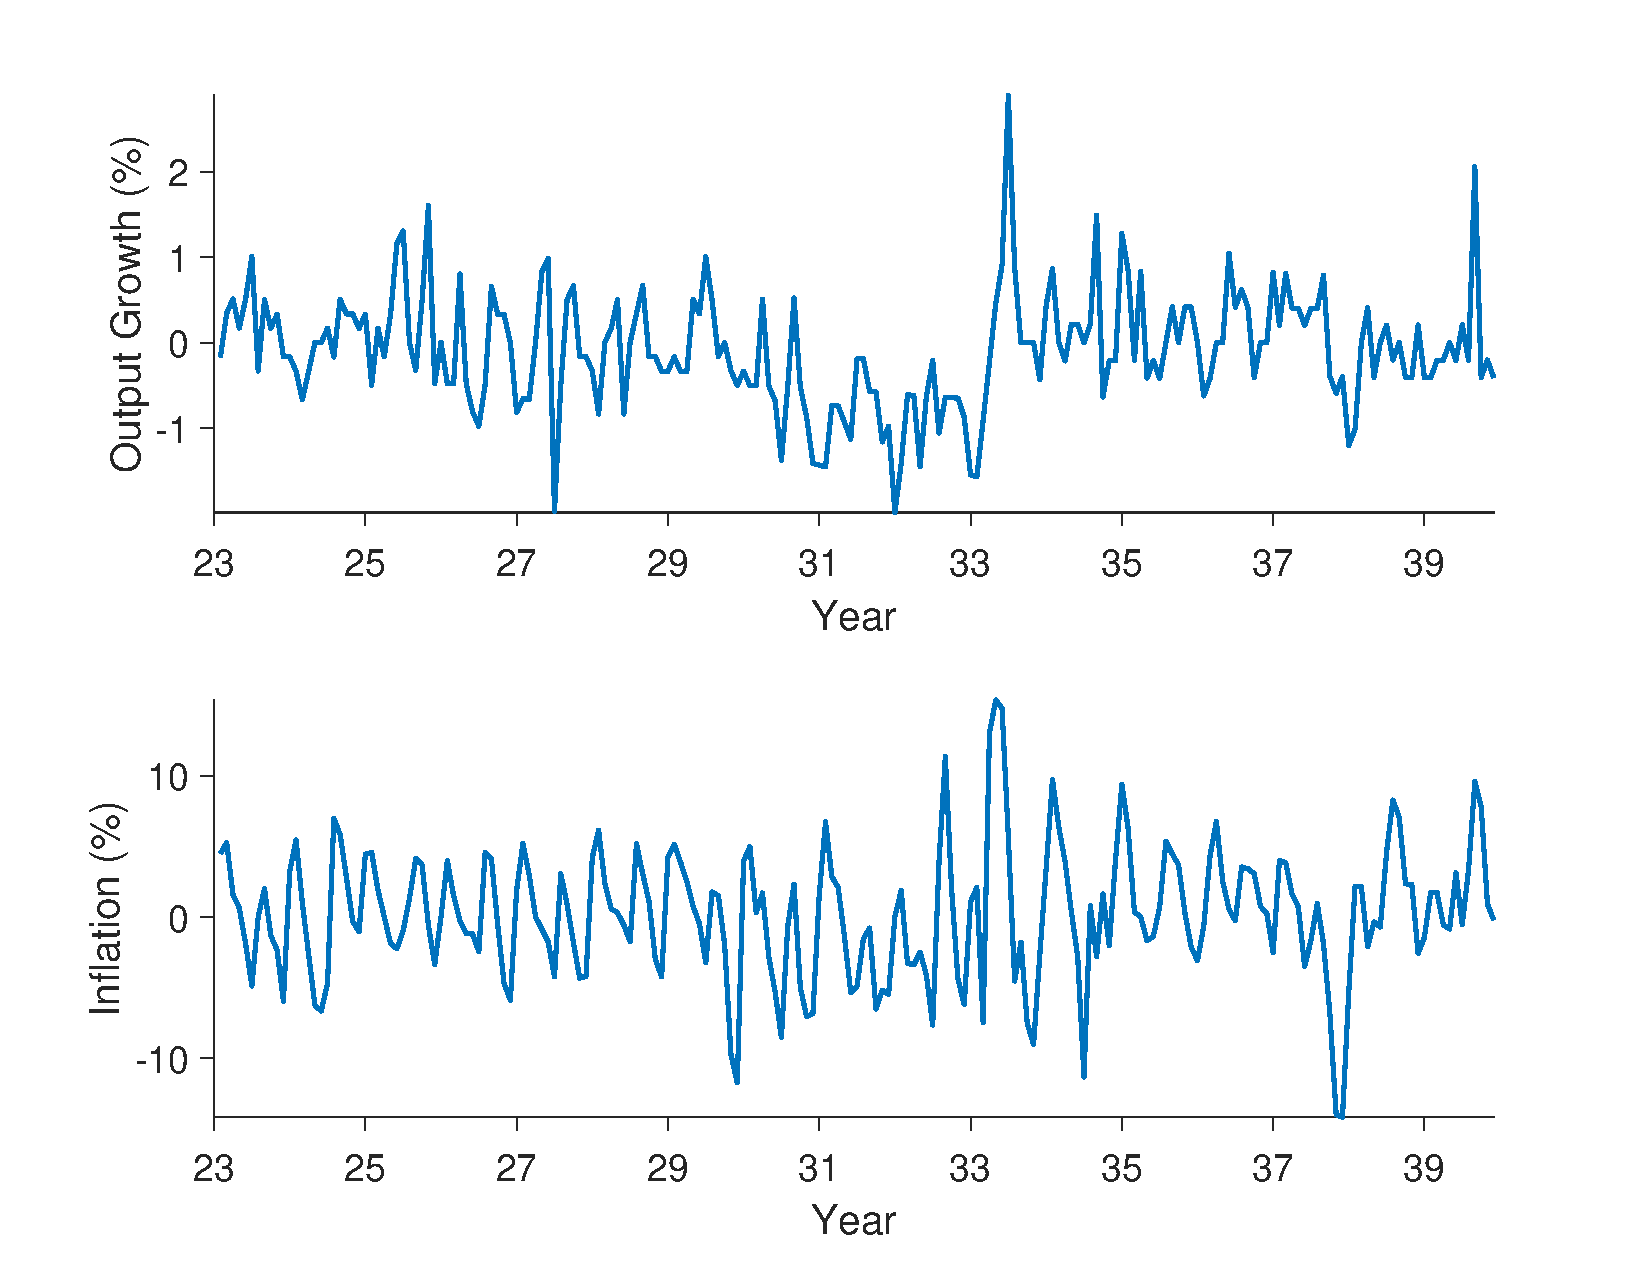
\includegraphics[width=1\textwidth]{../../out/figures/data_plot.pdf}
  \vspace{3mm}
  \caption[US Output Growth \textit{(Industrial Production)} and Inflation \textit{(Consumer Price Index)}]{\textbf{US Output Growth \textit{(Industrial Production)} and Inflation \textit{(Consumer Price Index)}} (Log First Differences)}
  \label{plot}
\end{figure}


%%%%%%%%%%%%%%%%%%%%%%%%%%%%%%%%%%%%%%%%%%%%%%%%%%%%%%%%%%%%%%%%%%%%%%%%%%%%%%%%%%%%%%%%%%%%%%%%%%%%%%%%%%%%%%%%%%%%%%%%%%%%%%%%%%%%%%%%%%%%%%%%%%%
%
%
%
%	3. Methodology
%
%
%%%%%%%%%%%%%%%%%%%%%%%%%%%%%%%%%%%%%%%%%%%%%%%%%%%%%%%%%%%%%%%%%%%%%%%%%%%%%%%%%%%%%%%%%%%%%%%%%%%%%%%%%%%%%%%%%%%%%%%%%%%%%%%%%%%%%%%%%%%%%%%%%%%
\clearpage
\section{Methodology}
\label{s:methodology}

\subsection{Structural vector autoregression}
\label{s:structural}

In structural models (see equation (\ref{e:var})) there often are no possibilities to observe shocks that are of structural nature. Autoregressive models (VAR) are then estimated as alternative (see equation (\ref{eq:var2})).
\begin{equation}
{\bf Gx_t}={\bf Dx_{t-1}}+{\bf \epsilon_t}
		\label{e:var}
\end{equation}
where $
{\bf x_t}
=
\begin{bmatrix}
\Delta p_t \\
\Delta y_t \\
\end{bmatrix}
,
\quad
{\bf x_{t-1}}
=
\begin{bmatrix}
\Delta y_{t-1} \\
\Delta p_{t-1} \\
\end{bmatrix}
\quad
\textrm{and}
\quad
{\bf \epsilon_t}
=
\begin{bmatrix}
\epsilon_{y,t} \\
\epsilon_{p,t} \\
\end{bmatrix}
$

${\bf x_t}$ is a 2$\times$1 vector featuring output growth and inflation.
\begin{equation}
	{\bf x_t} = {\bf A(L)x_{t-1}} + {\bf u_t}
\label{eq:var2}
\end{equation}
where
$
{\bf A(L)}
=
{\bf G^{-1}D}
\quad
\textrm{and}
\quad
{\bf u_t}
=
{\bf G^{-1}}
{\bf \epsilon_t}
$

Estimates for ${\bf A(L)}$, the residuals ${\bf u_t}$ and the covariance matrix ${\bf \sum}$ are obtained by OLS. Equation (\ref{eq:ma}) shows the $MA(\infty)$ representation of such VAR model.
\begin{equation}
{\bf x_t}
=
{\bf B(L)u_t}
\label{eq:ma}
\end{equation}
Rearranging equation (\ref{eq:ma}) yields:
\begin{equation}
{\bf u_t}
=
{\bf G^{-1}\epsilon_t}
=
{\bf S\epsilon_t}
\label{eq:response}
\end{equation}
Equation (\ref{eq:res}) depicts the covariance matrix of ${\bf u_t}$:
\begin{equation}
{\bf \sum} = E \big[ {\bf u_t u'_t} \big] = {\bf S}E \big[ {\bf \epsilon_t \epsilon'_t} \big] {\bf S'} = {\bf SS'}
\label{eq:res}
\end{equation}
${\bf \epsilon_t}$ is assumed to be mutually uncorrelated with a normalized variance of 1. Therefore $var({\bf \epsilon_t})={\bf I}$.
Resolving equation (\ref{eq:res}) yields the identification matrix ${\bf S}$ (impact matrix)\footnote{The impact matrix maps structural shocks into residuals}. 

\subsection{Blanchard-Quah decomposition}
\label{s:bq}
Implications of the traditional AS-AD model (\cite{favero}) assume supply shocks to have permanent and demand shocks to have temporary effects, on output whereas price effects are permanent for both, supply and demand shocks.

Blanchard-Quah decomposition (\cite{blanchard}) requires the implications of the traditional AS-AD model to be fulfilled (\cite{favero}). These implications are then sufficient to compute the long-run structural coefficient matrix:

\begin{equation}
\begin{bmatrix}
\Delta p_t \\
\Delta y_t \\
\end{bmatrix}
=
\begin{bmatrix}
(+) & 0 \\
(-) & (+) \\
\end{bmatrix}
\begin{bmatrix}
\epsilon^S  \\
\epsilon^S \\
\end{bmatrix}
\label{eq:lr}
\end{equation}
where: $
\begin{bmatrix}
(+) & 0 \\
(-) & (+) \\
\end{bmatrix}
=
{\bf C(1)}
\quad
\textrm{and}
\quad
\begin{bmatrix}
\epsilon^S  \\
\epsilon^S \\
\end{bmatrix}
=
{\bf \epsilon}$

${\bf C(1)}$ is lower triangular by restriction from the AS-AS model\footnote{as demand shocks have no long-run effects on output}. The long-run multiplier of the reduced form is denoted by:
\begin{equation}
{\bf B(1)}={\bf C(1)S^{-1}}
\label{eq:lrm}
\end{equation}
Choleski decomposition of (\ref{eq:chole}) leads to the long-run coefficient {\bf C(1)} which in turn facilitates the calculation of the identification matrix ${\bf S}={\bf B(1)^{-1}C(1)}$ and the structural moving average representation ${\bf x_t}={\bf C(L)\epsilon_t}={\bf B(L)S\epsilon_t}$.

\begin{equation}
  \begin{split}
		{\bf B}(1)\bs{\Sigma}{\bf B}(1)'=&{\bf C}(1){\bf S}^{-1}\bs{\Sigma}({\bf S}')^{-1}{\bf C}(1)'=\\=&{\bf C}(1){\bf S}^{-1}{\bf S}{\bf S}'({\bf S}')^{-1}{\bf C}(1)^		{\prime}=\\=&{\bf C}(1){\bf C}(1)'.
   \end{split}
\label{eq:chole}			
\end{equation}

\clearpage
%%%%%%%%%%%%%%%%%%%%%%%%%%%%%%%%%%%%%%%%%%%%%%%%%%%%%%%%%%%%%%%%%%%%%%%%%%%%%%%%%%%%%%%%%%%%%%%%%%%%%%%%%%%%%%%%%%%%%%%%%%%%%%%%%%%%%%%%%%%%%%%%%%%
%
%
%
%	4. Results
%
%
%%%%%%%%%%%%%%%%%%%%%%%%%%%%%%%%%%%%%%%%%%%%%%%%%%%%%%%%%%%%%%%%%%%%%%%%%%%%%%%%%%%%%%%%%%%%%%%%%%%%%%%%%%%%%%%%%%%%%%%%%%%%%%%%%%%%%%%%%%%%%%%%%%%
\section{Results}
\subsection{Impulse response functions}
\label{s:ir}
Figure (\ref{irt}) shows the impulse response functions \textit{(IR)} calculated on the basis off the entire dataset (years 1919-1939) . Figure (\ref{irr}) features impulse response functions on the \textit{Roaring Twenties} sub-sample (1920-1982). Figures (\ref{irg}) and (\ref{irn}) cover the \textit{Great Depression} (1929-1933) and the \textit{New Deal} era (1933-1937) respectively.

\begin{figure}[ht]
  \setstretch{1.0} 
  \footnotesize 
  \centering
  		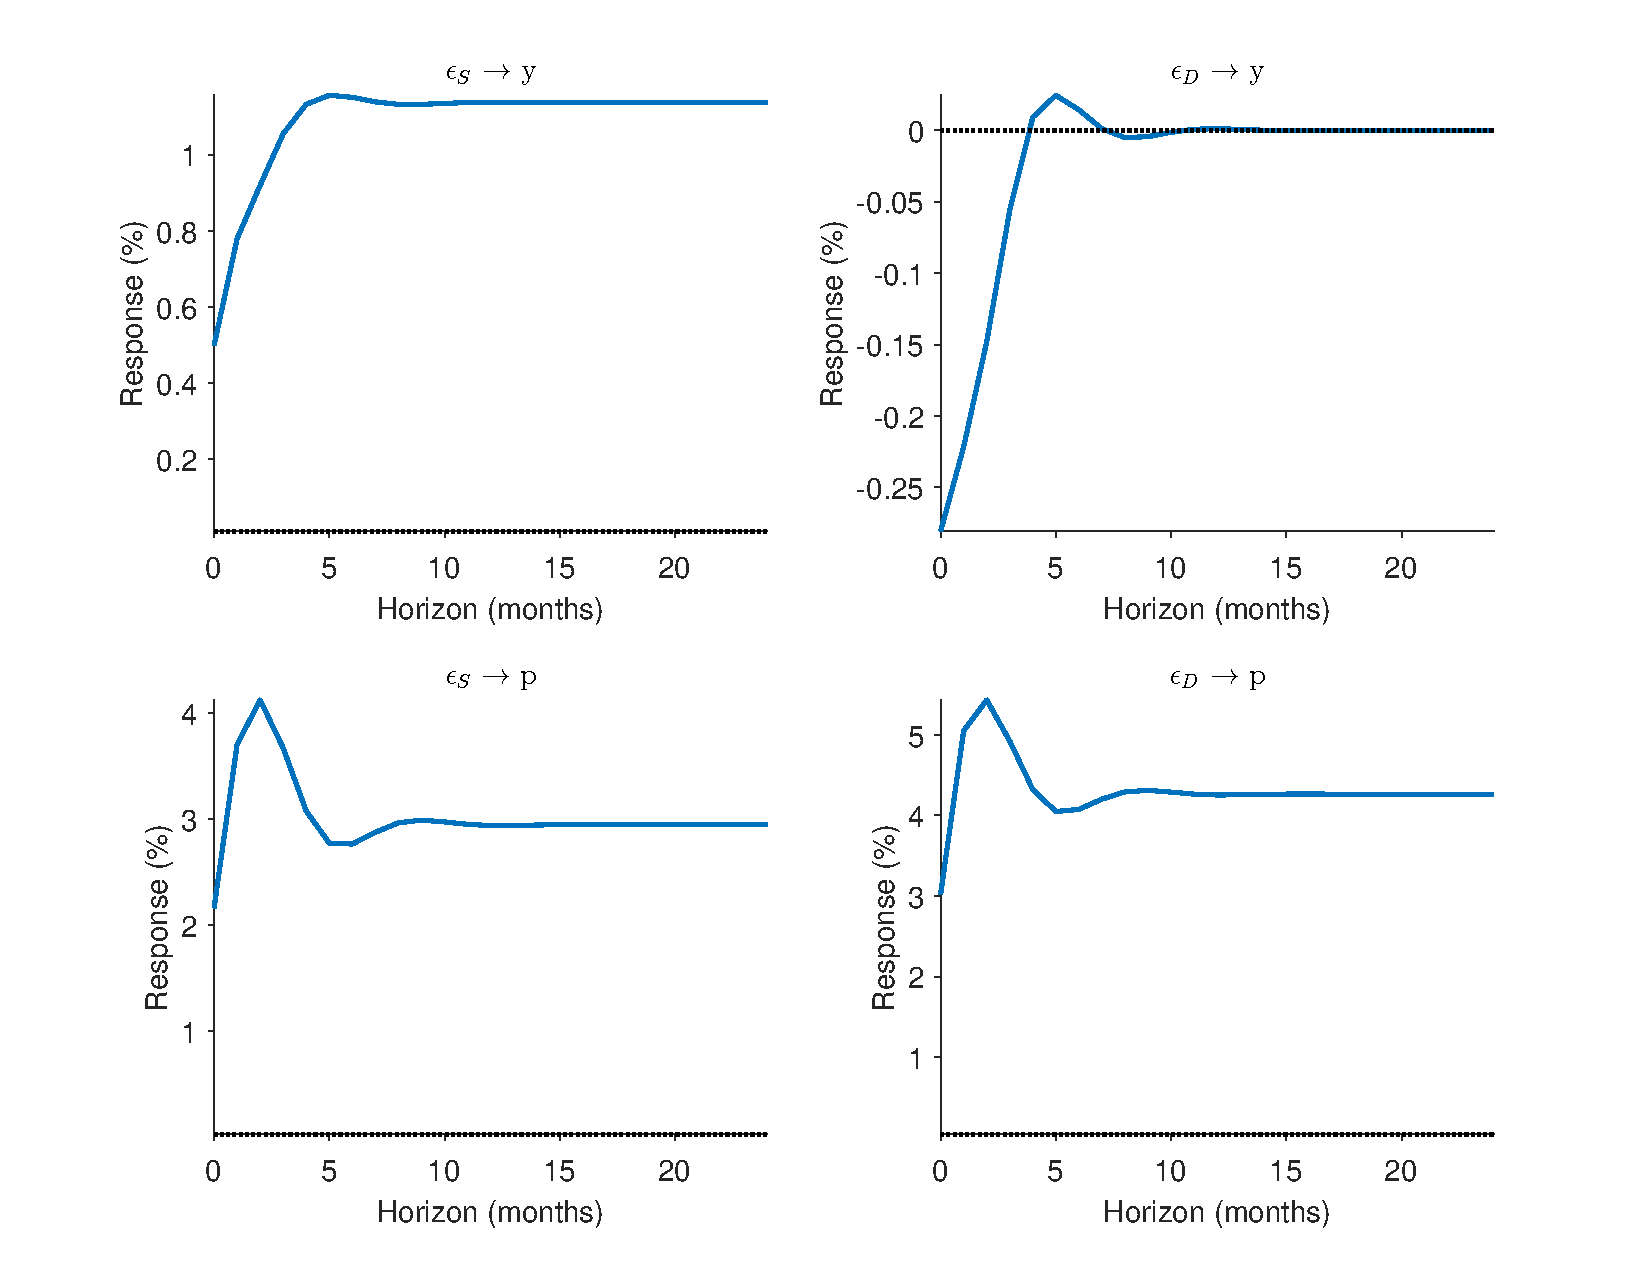
\includegraphics[width=1\textwidth]{../../out/figures/impulse_response.pdf}
  \vspace{3mm}
  \caption[Impulse response functions - entire dataset]{\textbf{Impulse response functions - entire dataset} (January 1919 - December 1939)}
  \label{irt}
\end{figure}

\begin{figure}[ht]
  \setstretch{1.0} 
  \footnotesize 
  \centering
  		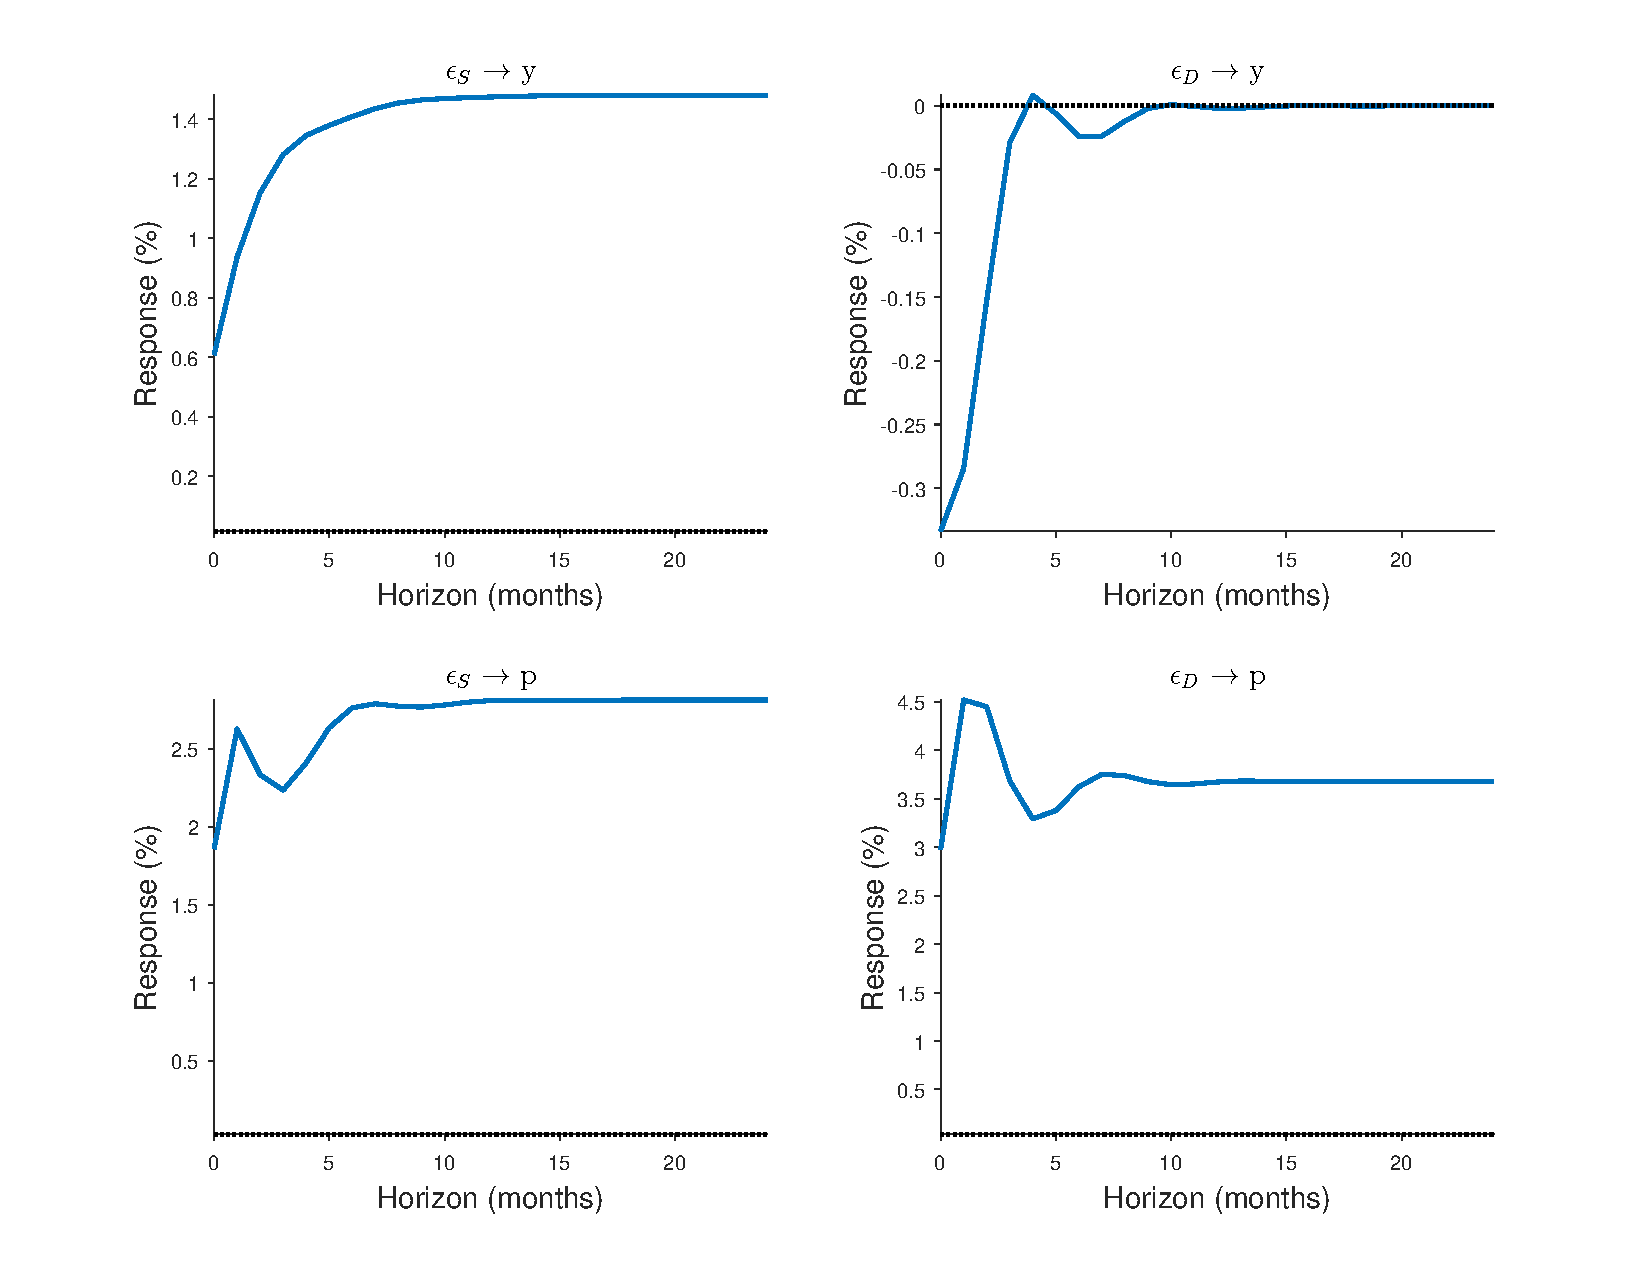
\includegraphics[width=1\textwidth]{../../out/figures/impulse_response_RT.pdf}
  \vspace{3mm}
  \caption[Impulse response functions - Roaring Twenties]{\textbf{Impulse response functions - Roaring Twenties} (January 1920 - December 1928)}
  \label{irr}
\end{figure}

\begin{figure}[ht]
  \setstretch{1.0} 
  \footnotesize 
  \centering
  		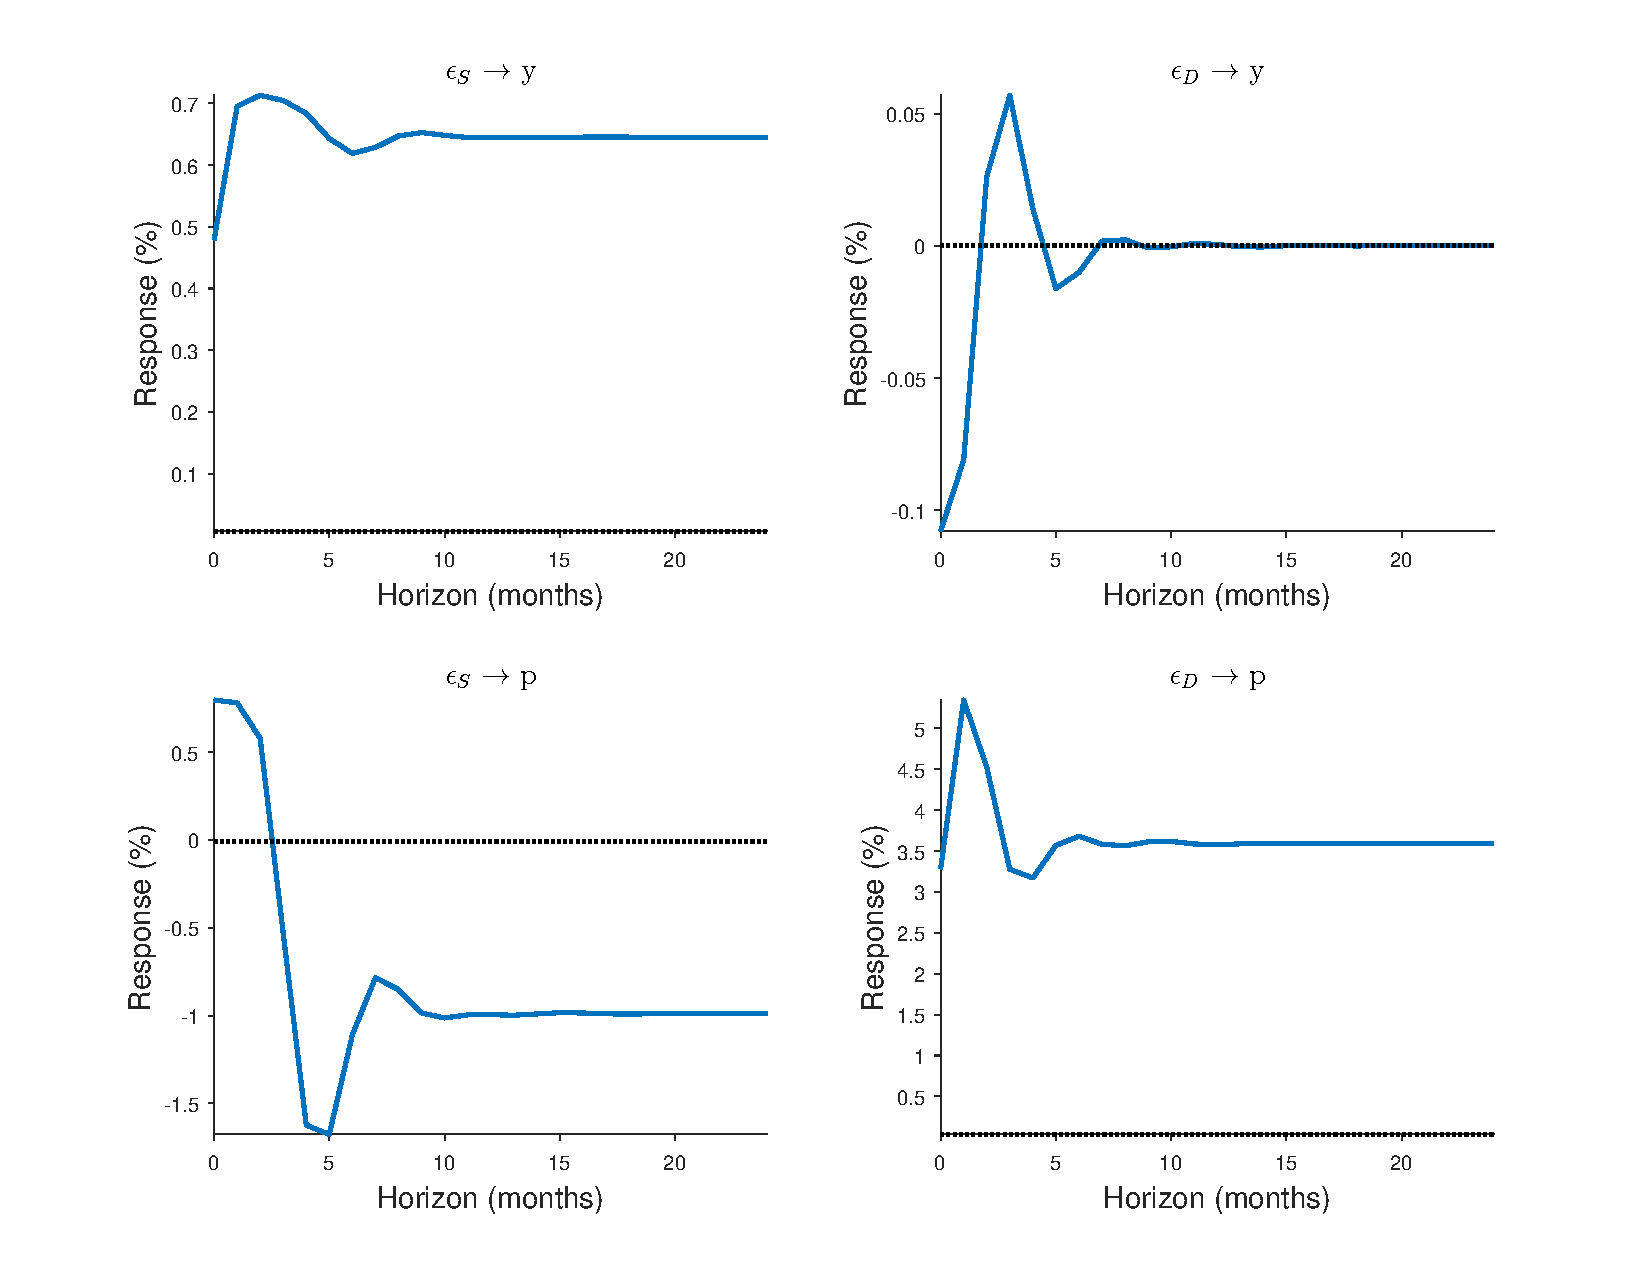
\includegraphics[width=1\textwidth]{../../out/figures/impulse_response_GD.pdf}
  \vspace{3mm}
  \caption[Impulse response functions - Great Depression]{\textbf{Impulse response functions - Great Depression} (October 1929 - February 1933)}
  \label{irg}
\end{figure}

\begin{figure}[ht]
  \setstretch{1.0} 
  \footnotesize 
  \centering
  		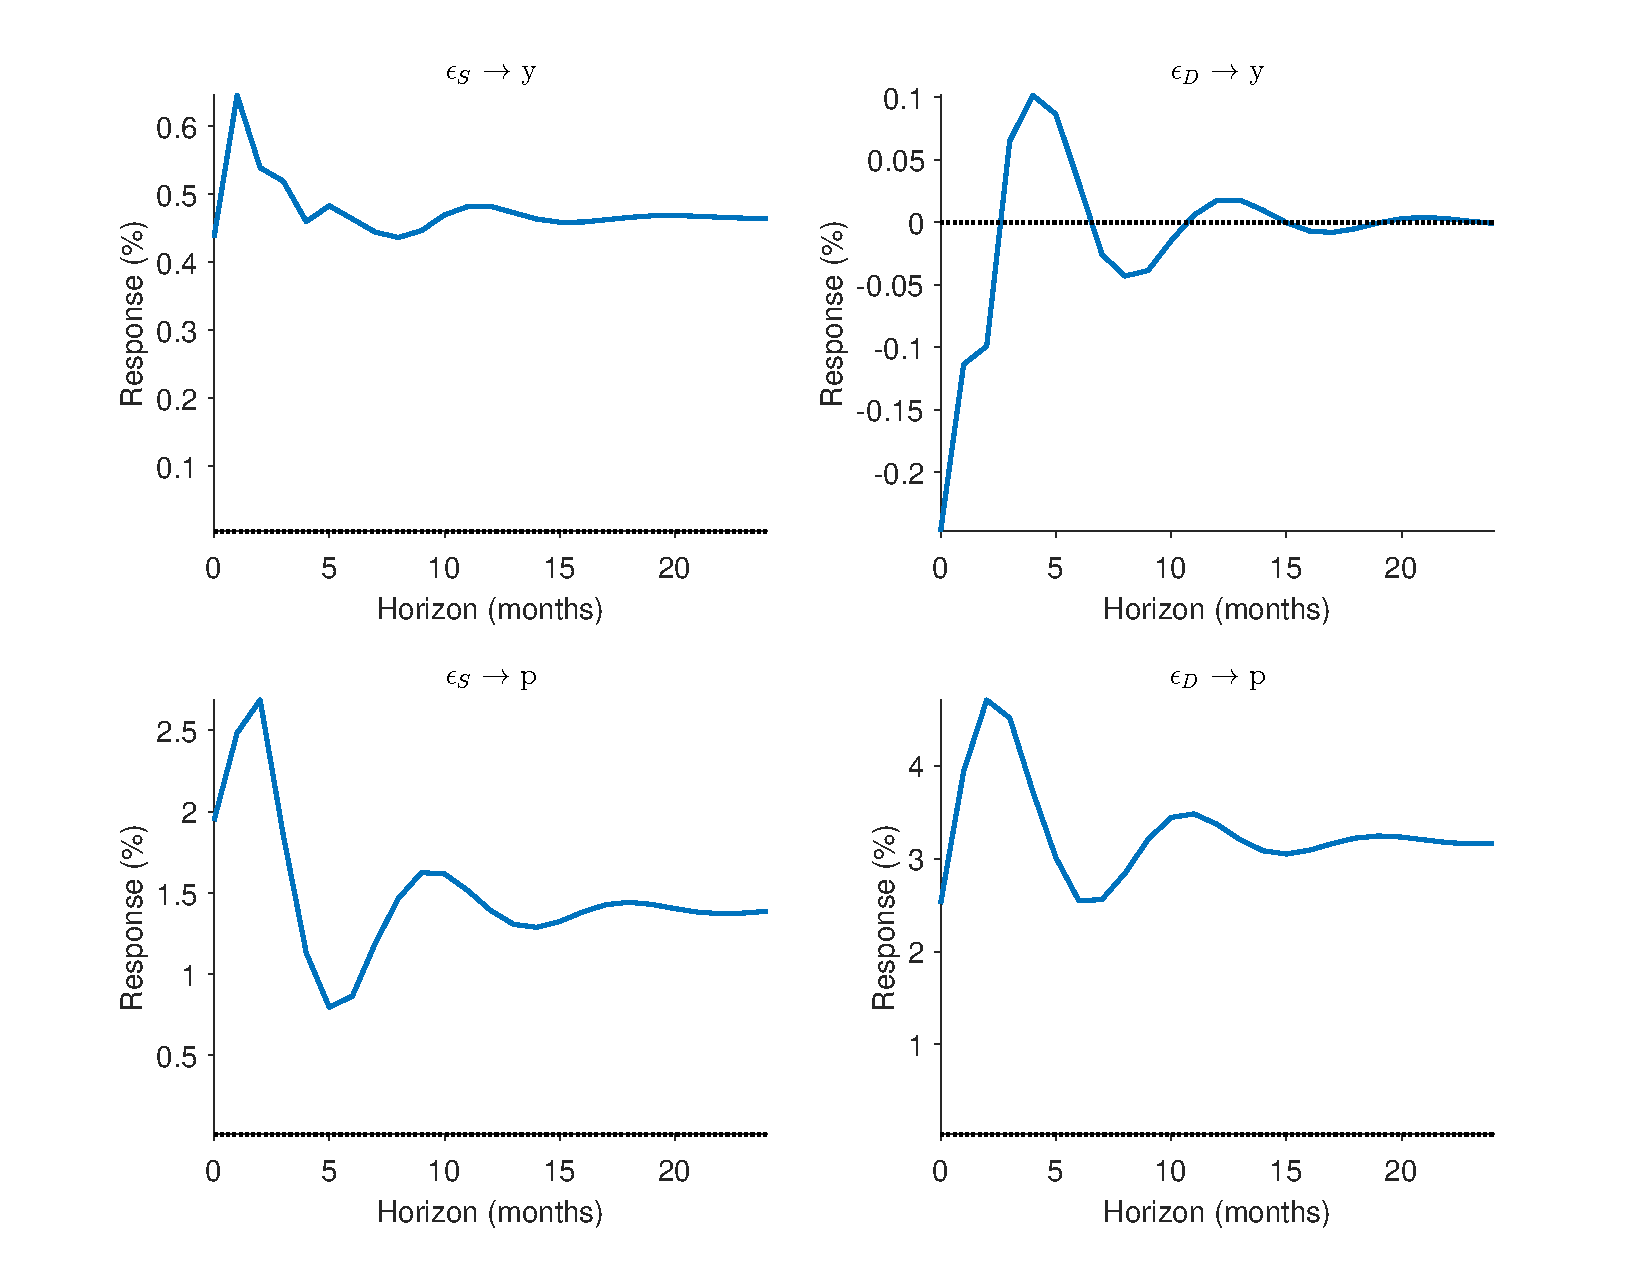
\includegraphics[width=1\textwidth]{../../out/figures/impulse_response_ND.pdf}
  \vspace{3mm}
  \caption[Impulse response functions - New Deal]{\textbf{Impulse response functions - New Deal} (April 1933 - June 1937)}
  \label{irn}
\end{figure}

The impulse response function indicate positive short-run output changes in response to a demand shock for the \textit{Great Depression} and \textit{New Deal} sub-samples. These reactions converge to zero in the long-run (which is in line with the restrictions imposed on the Blanchard-Quah decomposition (\cite{blanchard}). Several dependencies in line with the traditional AS-AD model can be observed. Prices tend to increase after a positive demand shock, whereas output tends to rise after positive supply shocks. Figure (\ref{irt}) shows negative short-run effects on output to positive demand shocks during the \textit{Roaring Twenties}. This result collides with the relationship assumed by the traditional AS-AD model.

\clearpage
\subsection{Forecast Error Variance Decomposition}
Figure (\ref{ft}) shows the forecast error variance decompositions of the impulse response functions covering the entire dataset, whereas figures (\ref{fr}), (\ref{fg}), (\ref{fg}) and (\ref{fn}) show the forecast error variance decompositions for the \textit{Roaring Twenties}, \textit{Great Depression} and \textit{New Deal} sub-sets respectively. The results indicate that variation in output is mainly driven by supply shocks whereas variation in prices is mainly driven by shocks in demand. As require by Blanchard-Quah specifications, long-run variation in output is entirely driven by supply shocks. In the short-run there seems to be no impact on output from demand shocks.

\begin{figure}[ht]
  \setstretch{1.0} 
  \footnotesize 
  \centering
  		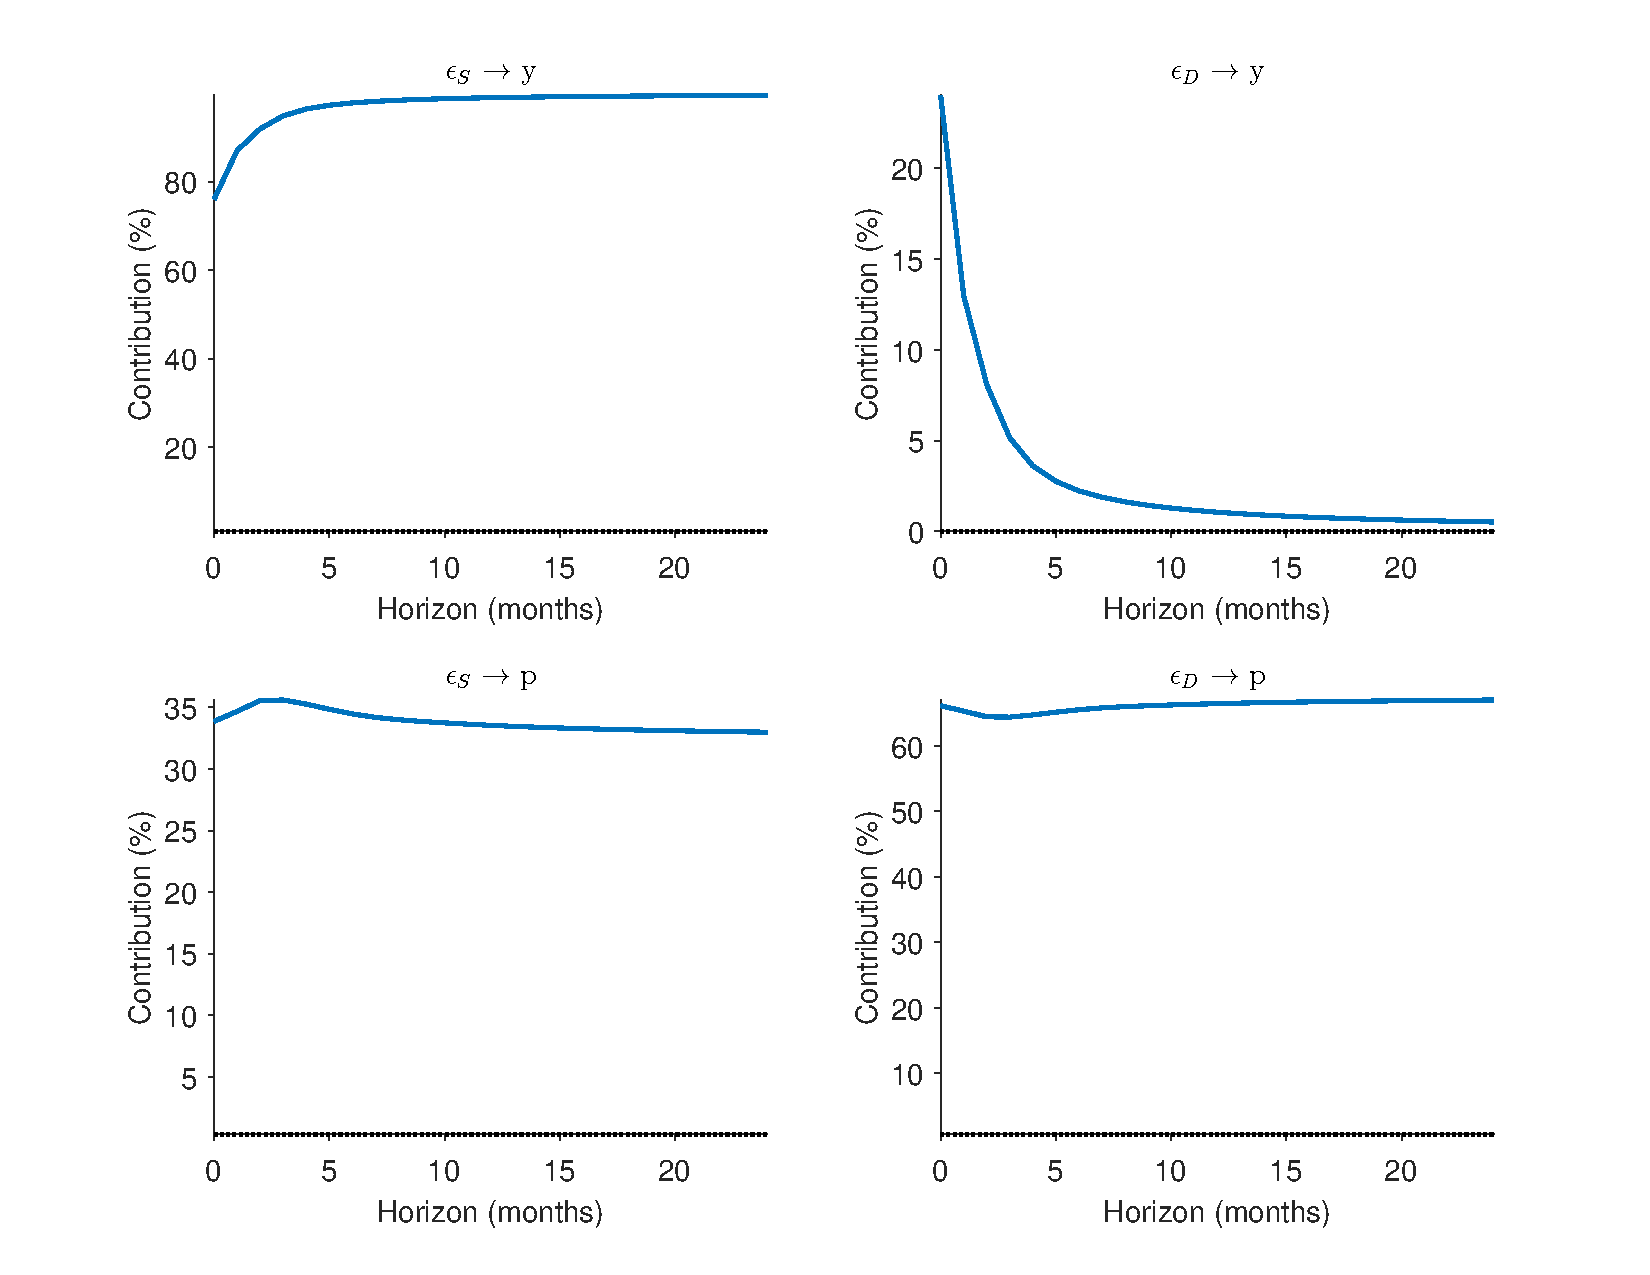
\includegraphics[width=1\textwidth]{../../out/figures/fevd.pdf}
  \vspace{3mm}
  \caption[Forecast error variance decomposition - Full data]{\textbf{Forecast error variance decomposition - entire dataset} (January 1919 - December 1939)}
  \label{ft}
\end{figure}

\begin{figure}[ht]
  \setstretch{1.0} 
  \footnotesize 
  \centering
  		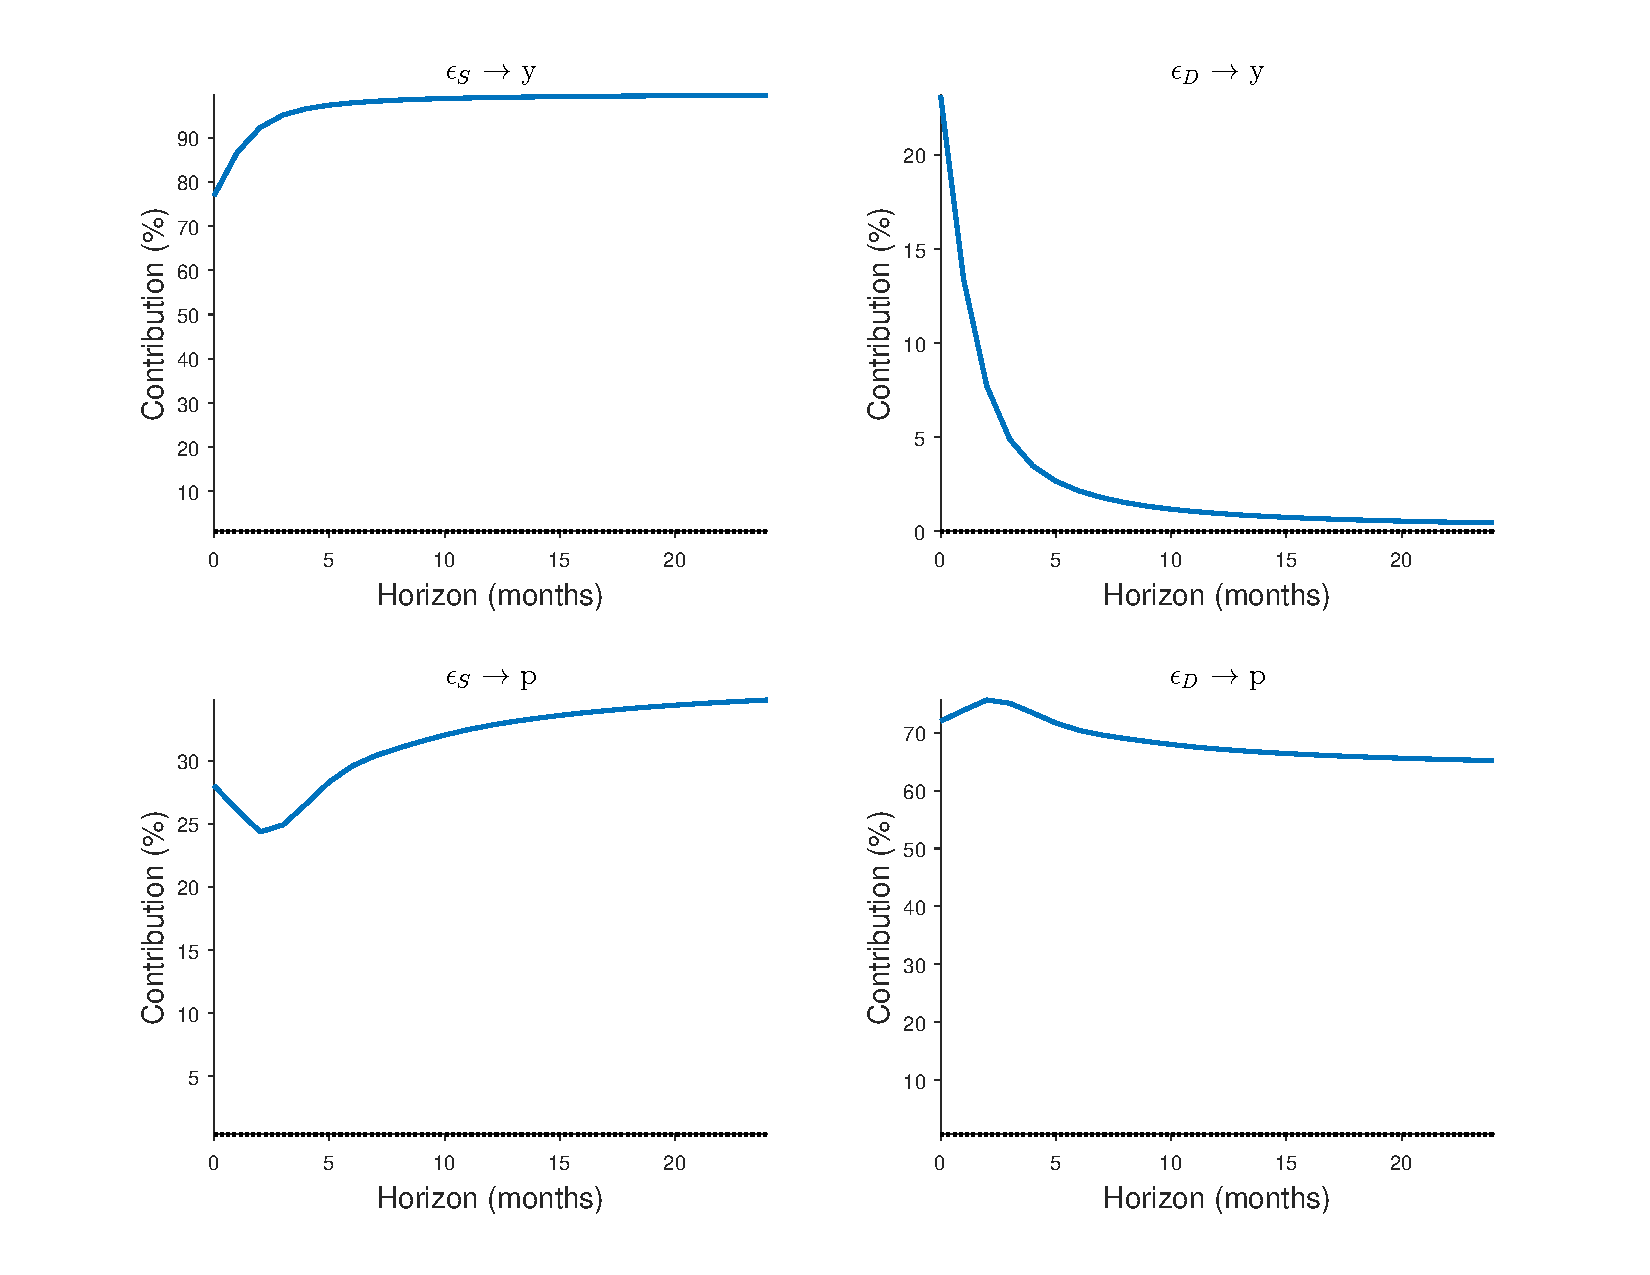
\includegraphics[width=1\textwidth]{../../out/figures/fevd_RT.pdf}
  \vspace{3mm}
  \caption[Forecast error variance decomposition - Roaring Twenties]{\textbf{Forecast error variance decomposition - Roaring Twenties} (January 1920 - December 1928)}
  \label{fr}
\end{figure}

\begin{figure}[ht]
  \setstretch{1.0} 
  \footnotesize 
  \centering
  		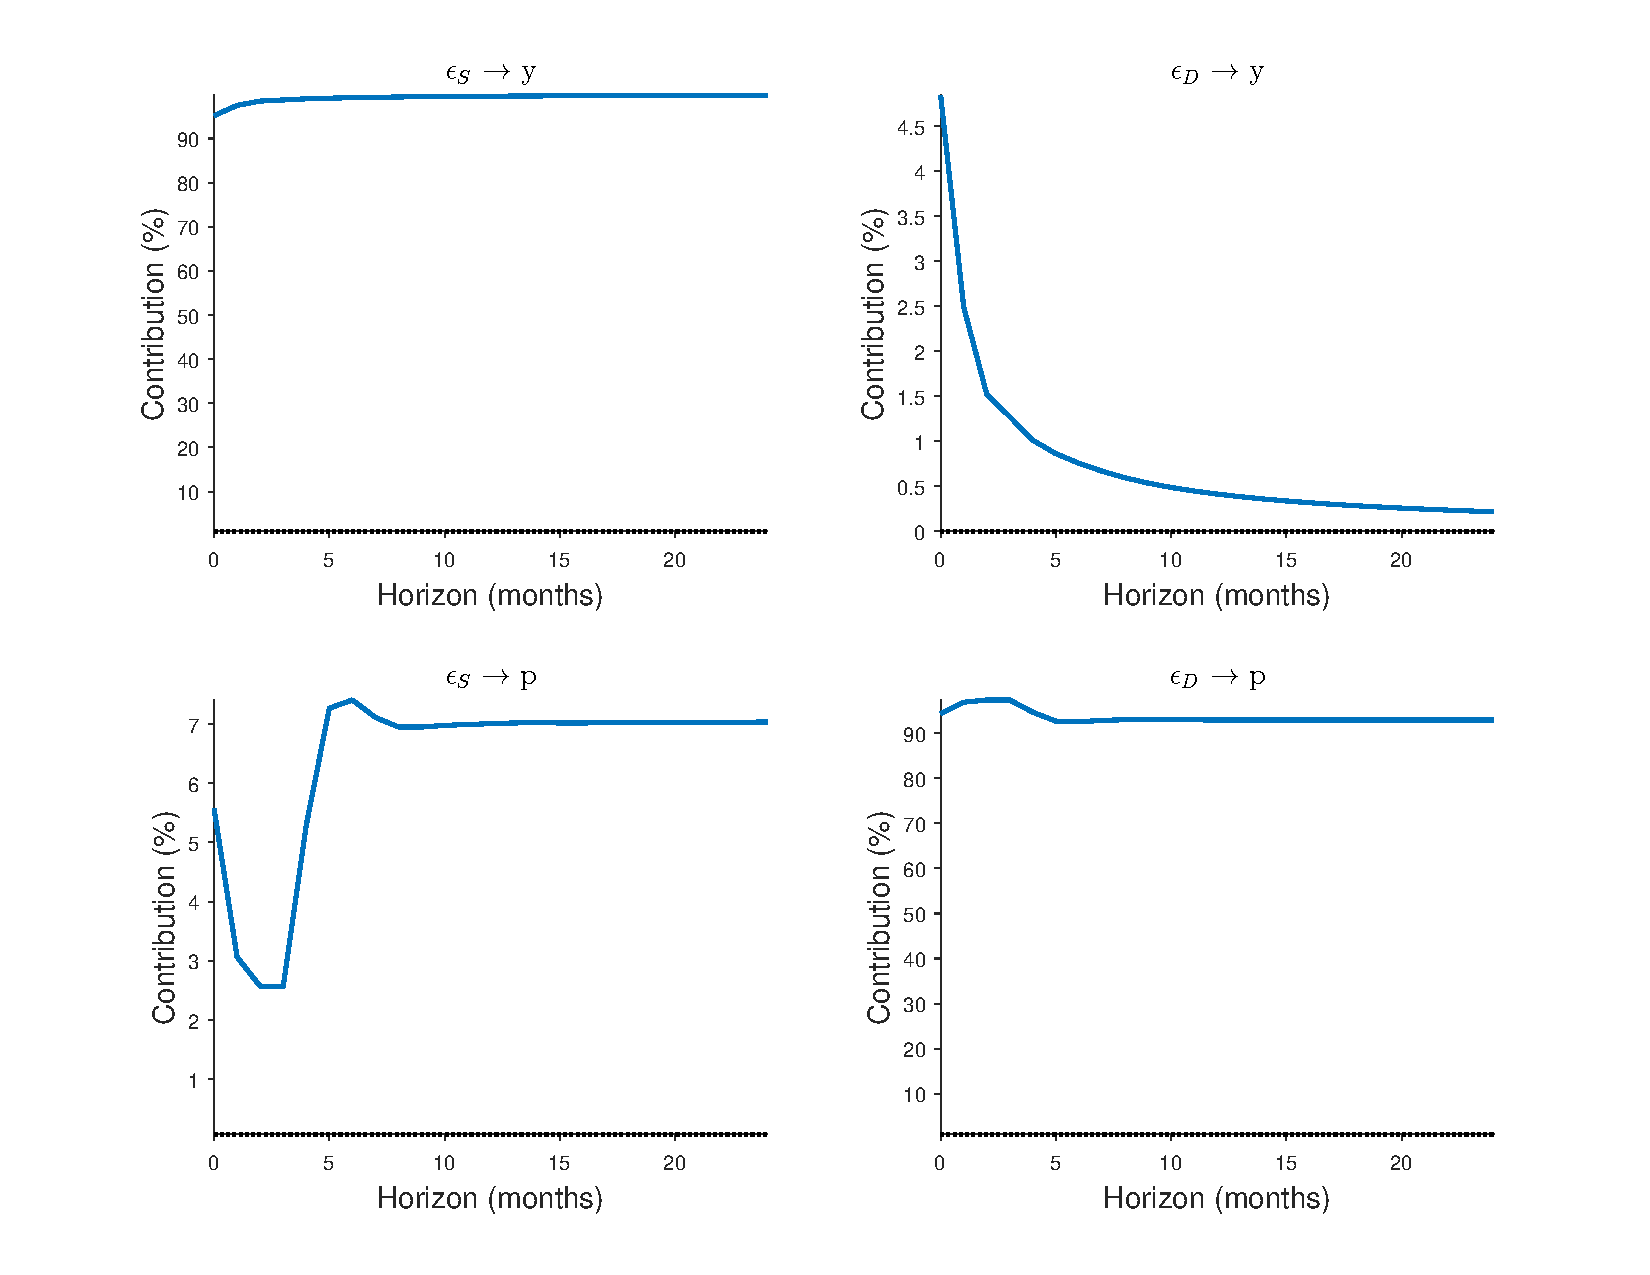
\includegraphics[width=1\textwidth]{../../out/figures/fevd_GD.pdf}
  \vspace{3mm}
  \caption[Forecast error variance decomposition - Great Depression]{\textbf{Forecast error variance decomposition - Great Depression} (October 1929 - February 1933)}
  \label{fg}
\end{figure}

\begin{figure}[ht]
  \setstretch{1.0} 
  \footnotesize 
  \centering
  		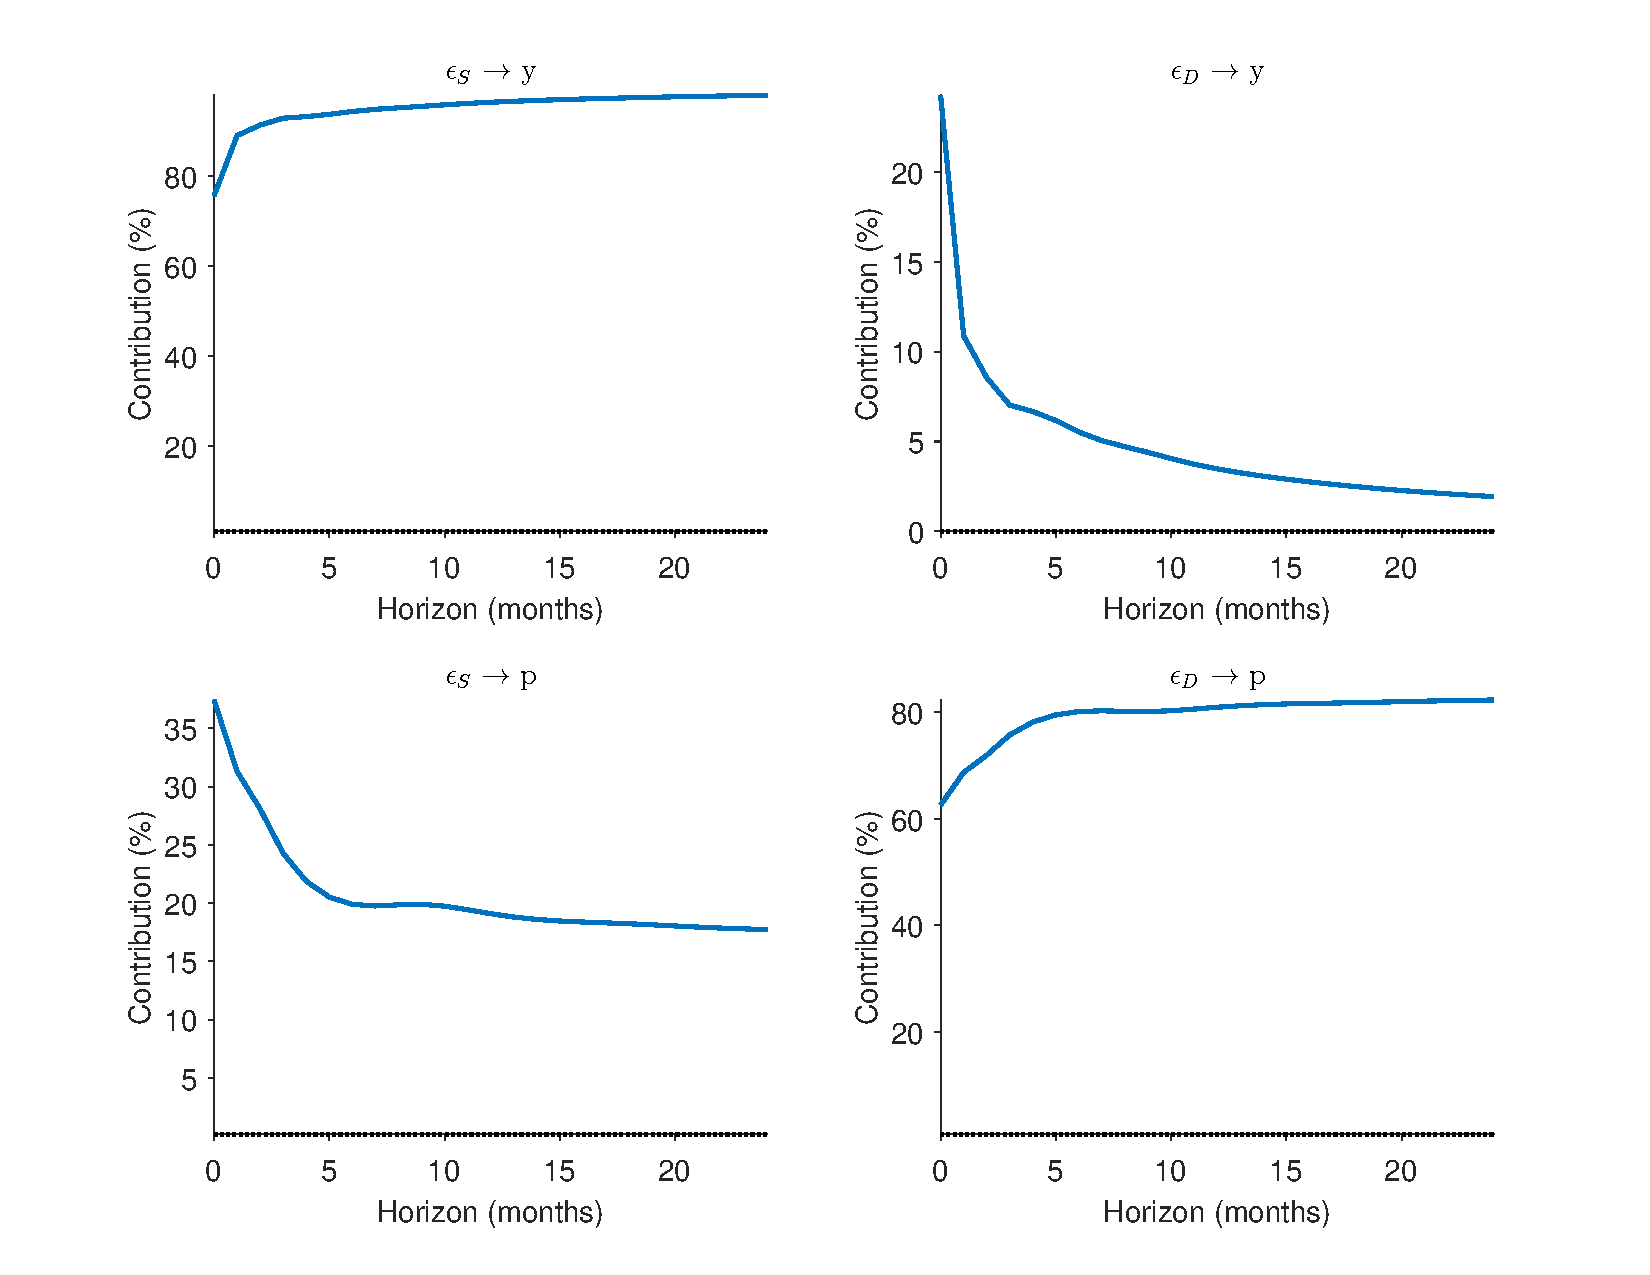
\includegraphics[width=1\textwidth]{../../out/figures/fevd_ND.pdf}
  \vspace{3mm}
  \caption[Forecast error variance decomposition - New Deal]{\textbf{Forecast error variance decomposition - New Deal} (April 1933 - June 1937)}
  \label{fn}
\end{figure}

\clearpage

\section{Conclusion}
In general Blanchard-Quah decompositions lead to results further in line with textbook macroeconomic models when applied to post-World War II data (see e.g. \cite{blanchard2}). Applying Blanchard-Quah decomposition on the evaluated dataset may lead to several implications that seem counterfactual to the traditional AS-AD model (see section \ref{s:ir}). Blanchard-Quah decompositions seem to be of limited power when modelling the effects of structural shocks that occurred in the \textit{inter war} period (see e.g. \cite{eggertson} who claim that monopoly protection and union support backed by \textit{New Deal} policies were beneficial to output growth or \cite{comm} who highlight the effects of commodity markets disintegration after 1929). 


